Using logic grid puzzles as a use-case, we will validate the feasibility of finding a sequence of small explanations.

As data we use puzzles from Puzzle Baron’s Logic Puzzles Volume 3~\cite{logigrammen}. The first 10 puzzles were used to construct the grammar. Using this grammar, and a semi-automatically problem-specific lexicon, we are able to parse and solve all puzzles in the booklet, including those not used to construct the grammar. Our experiments below are on test puzzles not used to construct the grammar; we also report results on the \textit{pasta} puzzle, which was emailed to us by a person that did not manage to solve it himself.\tias{do we know the source of the original puzzle?}

As constraint solving engine, we use IDP~\cite{idp}. It is a knowledge representation and reasoning system that supports multiple queries on a first order logic theory. We will use the 'optimalpropagate()' query, which efficiently finds the maximally consistent (partial) interpretation of a theory, which in our case is a full interpretation, e.g. the solution to the logic grid puzzle. We also use the 'findMUS()'\tias{Bart, how is it really name?} query that searches for a subset-minimal unsatisfiable core.

The algorithm itself is written in embedded LUA, which is provided as en imperative environment inside the otherwise declarative IDP system. The code was not optimized for efficiency and can at this point not be used in an interactive setting, as it takes between 15 minutes to a few hours to fully explain a logic grid puzzle. Experiments were run on an Intel(R) Xeon(R) CPU E3-1225 with 4 cores and 32 Gb memory, running linux 4.15.0 and IDP version 3.7.1.


We analyze the results in 3 directions :

\paragraph{Q1. How do different puzzles compare with respect to the generated explanations ?} For future reference, we denote \textbf{c} = $c_1, c2, ...c_n$ the costs, where $c_i$ is the cost, based on the cost function $f(I, C)$, at reasoning step $i$ and n the number of reasoning steps to solve a problem. Table \ref{table:sequence_leve} shows how difficult the puzzles are by means of the total cost and how the expensive a new conclusion is based on the current state of the grid.


\begin{table}
	\centering
	\resizebox{\columnwidth}{!}{%
\begin{tabular}{cccc|cccccc}
n & $|type|$ & $|dom|$ & $|grid|$ & steps & \#bij & \#trans & \#clue & \#m-i & \#m-c \\ 
\hline 
%p5 & 113 & 626 & 25 & 5.59 & [25, 21, 21, 21, 21] & 31.0 & 50.0 & 0 & 19.0 & 0 \\ 
1 &  &  &  	& 113 & 31\% & 50\% & 19\% & 0 & 0 \\ 
%p16 & 122 & 680 & 23 & 5.62 & [23, 21, 21, 21, 21] & 21.0 & 60.0 & 0 & 19.0 & 0 \\ 
%p93 & 119 & 659 & 21 & 5.58 & [21, 21, 21, 21, 20] & 34.0 & 47.0 & 0 & 19.0 & 0 \\ 
%\textbf{p12} & \textbf{115} & \textbf{591} & \textbf{23} & \textbf{5.18} & \textbf{[23, 21, 21, 21, 20]} & \textbf{29.0} & \textbf{54.0} & \textbf{0} & \textbf{17.0} & \textbf{0} \\ 
%\textbf{p18} & \textbf{116} & \textbf{615} & \textbf{22} & \textbf{5.35} & \textbf{[22, 22, 22, 21, 21]} & \textbf{28.0} & \textbf{55.0 }& \textbf{0 }& \textbf{17.0} & \textbf{0 }\\ 
%p20 & 116 & 552 & 22 & 4.8 & [22, 21, 21, 21, 20] & 27.0 & 58.0 & 0 & 15.0 & 0 \\ 
%\textbf{p25} & \textbf{111} & \textbf{595} & \textbf{24} & \textbf{5.41} & \textbf{[24, 23, 22, 21, 21]} & \textbf{37.0} & \textbf{45.0} & \textbf{0} &\textbf{ 17.0} & \textbf{0} \\ 
%p19 & 123 & 630 & 22 & 5.16 & [22, 21, 21, 21, 21] & 25.0 & 59.0 & 0 & 16.0 & 0 \\ 
\hline

\end{tabular} 
	}
\caption{smth}
\label{table:smth}
\end{table}


$|type|$ = nr types
$|dom|$ = nr doms
$|grid|$ = $|dom|^2 * (|type|*(|type|-1)/2)$

\begin{table}
	\centering
	\resizebox{\columnwidth}{!}{%
\begin{tabular}{|c||c|c|c|c|c||c|c|c|c|c|c|} 
\hline 
\textbf{Puzzle} & \textbf{n} & $\sum_{i = 1}^{n} c_i$  & max(\textbf{c}) & $\overline{\text{\textbf{c}}}$ & \textbf{5 Highest costs} & \textbf{\% bij.} & \textbf{\% trans.} & \textbf{\% comb.} & \textbf{\% clue} & \textbf{\% multi. clues} \\ 
\hline 
p5 & 113 & 626 & 25 & 5.59 & [25, 21, 21, 21, 21] & 31.0 & 50.0 & 0 & 19.0 & 0 \\ 
\hline 
p16 & 122 & 680 & 23 & 5.62 & [23, 21, 21, 21, 21] & 21.0 & 60.0 & 0 & 19.0 & 0 \\ 
\hline 
p93 & 119 & 659 & 21 & 5.58 & [21, 21, 21, 21, 20] & 34.0 & 47.0 & 0 & 19.0 & 0 \\ 
\hline 
\textbf{p12} & \textbf{115} & \textbf{591} & \textbf{23} & \textbf{5.18} & \textbf{[23, 21, 21, 21, 20]} & \textbf{29.0} & \textbf{54.0} & \textbf{0} & \textbf{17.0} & \textbf{0} \\ 
\hline 
\textbf{p18} & \textbf{116} & \textbf{615} & \textbf{22} & \textbf{5.35} & \textbf{[22, 22, 22, 21, 21]} & \textbf{28.0} & \textbf{55.0 }& \textbf{0 }& \textbf{17.0} & \textbf{0 }\\ 
\hline 
p20 & 116 & 552 & 22 & 4.8 & [22, 21, 21, 21, 20] & 27.0 & 58.0 & 0 & 15.0 & 0 \\ 
\hline 
\textbf{p25} & \textbf{111} & \textbf{595} & \textbf{24} & \textbf{5.41} & \textbf{[24, 23, 22, 21, 21]} & \textbf{37.0} & \textbf{45.0} & \textbf{0} &\textbf{ 17.0} & \textbf{0} \\ 
\hline 
p19 & 123 & 630 & 22 & 5.16 & [22, 21, 21, 21, 21] & 25.0 & 59.0 & 0 & 16.0 & 0 \\ 
\hline
\end{tabular} 
	}
\caption{Puzzle explanation cost based on the cost function $f(I, C)$ and statistics on puzzle constraints}
\label{table:sequence_leve}
\end{table}

While the first part of the table \ref{table:sequence_leve} only analyzes the difficulty of a puzzle, the second part focuses on the explanations. 
Most of the explanations are either generated using bijectivity (bij.) or Transitivity (trans.). The rest are found using the 1 or more clues, or by combining (comb.) transitivity with bijectivity. This is due to the way puzzles are formulated in natural language for logic grid puzzles.

\paragraph{Q2. How does the level of difficulty progress throughout the explanation?} Out of the problems in table \ref{table:sequence_leve}, 3 puzzle instances were selected: \textit{p12}, \textit{p18} and \textit{p25}. These puzzles present a similar number of explanation steps and total costs.

\begin{figure}
	\centering
	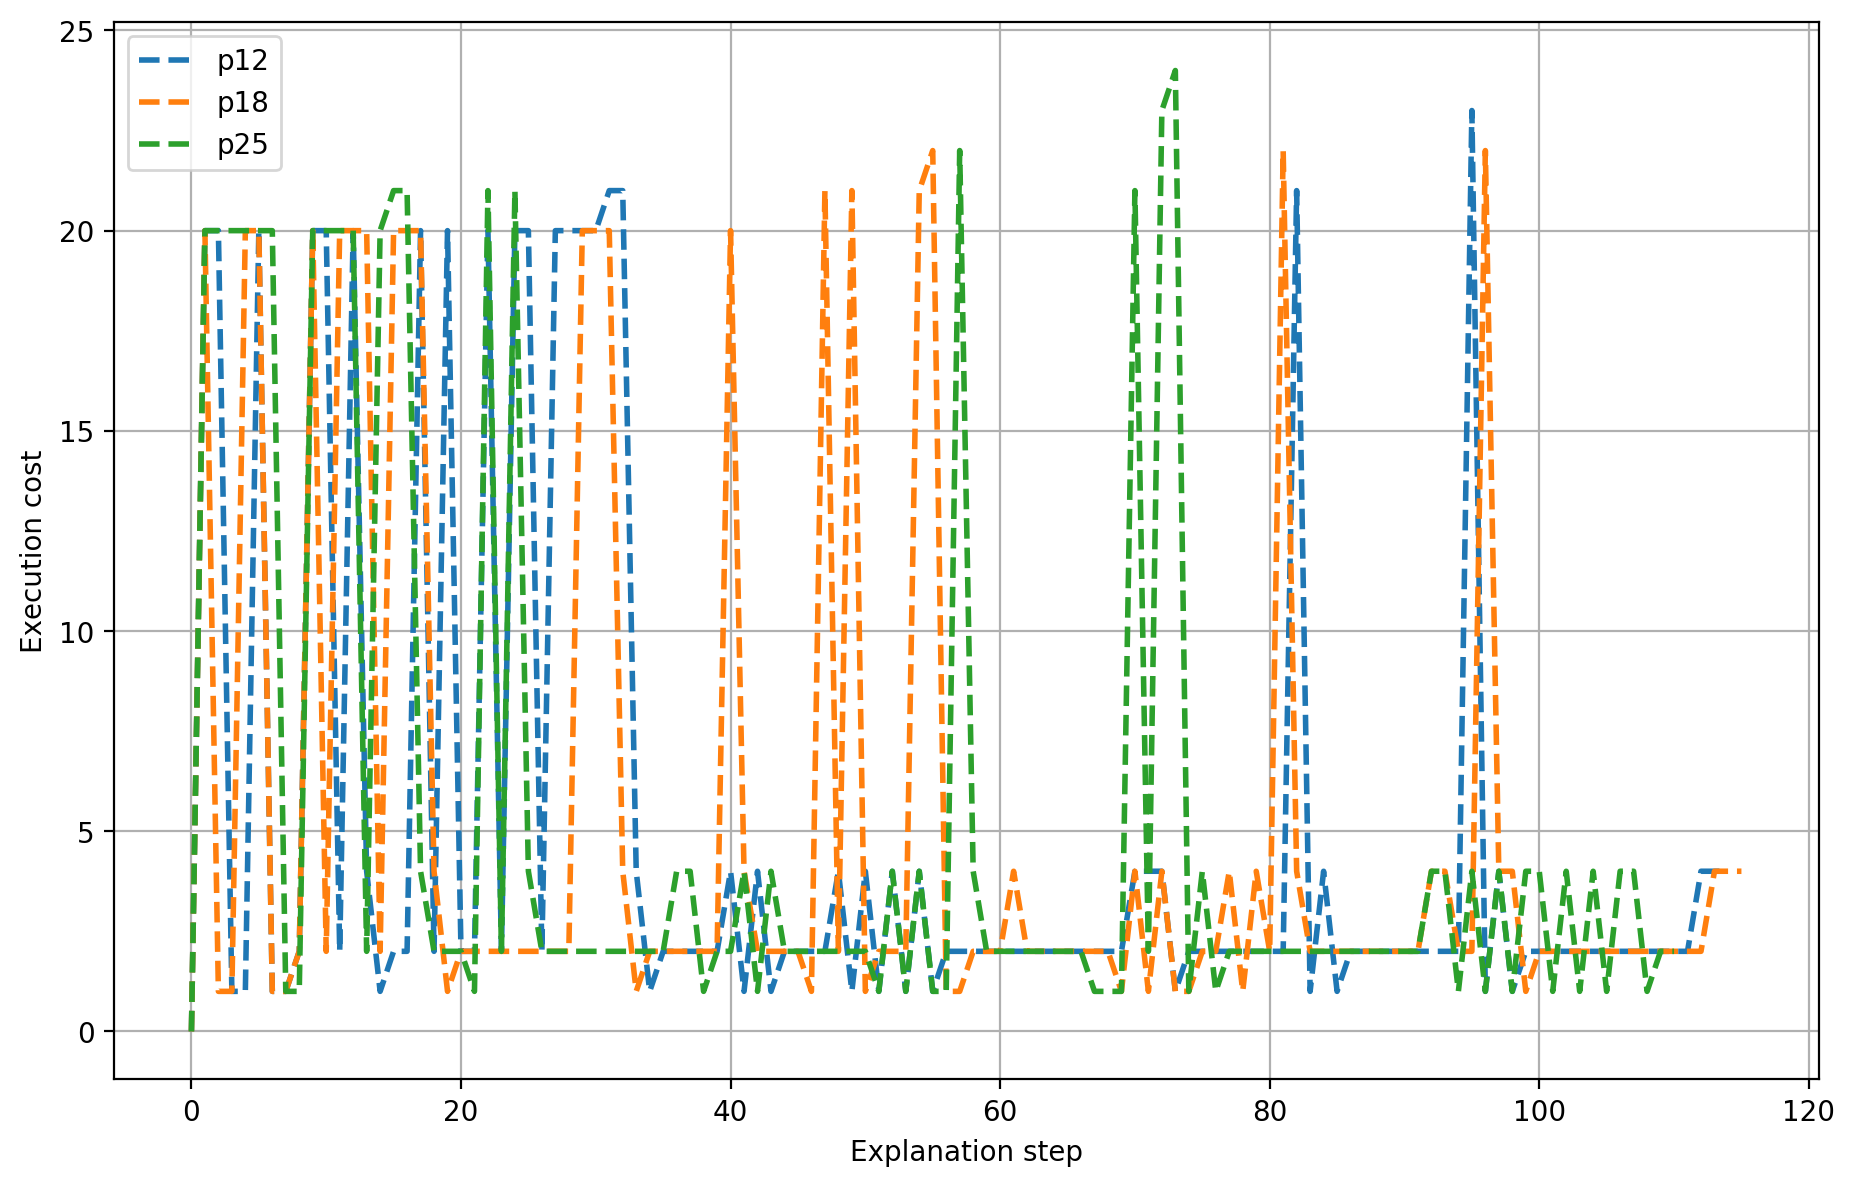
\includegraphics[width=0.7\linewidth]{figures/plot_cost_steps.png}
		\caption{Explanation cost for puzzle instances p12, p18, p25}
			\label{fig:plotcoststeps}
\end{figure}

\begin{table}
	\centering
	\resizebox{\columnwidth}{!}{%
		\begin{tabular}{|l||c|c|c|c|c|c|c|} 
			\hline
			\textbf{puzzle} & \textbf{tot exec time} & avg clue time  & avg bij. & avg trans. & avg time/cost of clue & avg time/cost of bij. & avg time/cost of bij. \\ 
			\hline 
			p5 & 386.0 & 129.29 & 226.27 & 204.23 & 6.13 & 145.18 & 102.11 \\ 
			\hline 
			p16 & 576.0 & 192.97 & 370.55 & 426.41 & 9.22 & 213.63 & 213.21 \\ 
			\hline 
			p93 & 946.0 & 213.13 & 604.13 & 425.58 & 10.44 & 340.27 & 212.79 \\ 
			\hline 
			p12 & 1103.0 & 271.13 & 744.93 & 799.79 & 12.87 & 432.21 & 399.89 \\ 
			\hline 
			p18 & 1924.0 & 323.82 & 856.52 & 881.44 & 15.14 & 421.34 & 440.72 \\ 
			\hline 
			p20 & 411.0 & 117.57 & 235.34 & 235.29 & 5.69 & 147.65 & 117.64 \\ 
			\hline 
			p25 & 886.0 & 291.12 & 659.88 & 623.77 & 13.42 & 404.61 & 311.89 \\ 
			\hline 
			p19 & 1207.0 & 265.82 & 538.64 & 602.01 & 12.77 & 293.38 & 301.0 \\ 
			\hline 
		\end{tabular} 
	}
	\caption{Puzzle explanation cost based on the cost function $f(I, C)$ and statistics on puzzle constraints}
	\label{table:sequence_leve}
\end{table}


\paragraph{Q3. How is the performance and the level of difficulty affected by removing parts of the algorithm ? } bla bla bla

% TODO table : Leaving some parts of the algo out, to see step-wise improvements of the components?  Some experiment with different levels of abstraction (e.g. all constraints at once, clues separate but all implicit at once, 2 groups of implicits, full split of implicits) with 'set of measures', so probably a table

\paragraph{Bonus. How well does it compare to human solving process ?} 

% TODO Compare with the tutorial puzzle of logicgridpuzzles.com? Ideally, a small human evaluation (e.g. ask people to solve a 3-with-3 puzzle and note the order of derivations and clues used, compare this 'ranking' to our ranking, discuss some differences.

\begin{table}
	\centering
	\resizebox{\columnwidth}{!}{%
		\begin{tabular}{|l||c|c|c|c|} 
			\hline 
			\textbf{puzzle} & \textbf{avg. fact used} & \textbf{avg. facts used with a clue} & \textbf{avg. facts used with trans.} & \textbf{avg. facts used together with bij.}\\ 
			\hline 
			p5.output.json & 1.823 & 0.524 & 2.371 & 2.0 \\ 
			\hline 
			p16.output.json & 1.803 & 0.609 & 2.385 & 2.0 \\ 
			\hline 
			p93.output.json & 1.84 & 0.182 & 2.575 & 2.0 \\ 
			\hline 
			p12.output.json & 1.835 & 0.316 & 2.455 & 2.0 \\ 
			\hline 
			p18.output.json & 1.853 & 0.45 & 2.5 & 2.0 \\ 
			\hline 
			p20.output.json & 1.828 & 0.294 & 2.355 & 2.0 \\ 
			\hline 
			nielspasta.output.json & 1.768 & 1.05 & 2.071 & 2.0 \\ 
			\hline 
			p25.output.json & 1.937 & 0.737 & 2.463 & 2.0 \\ 
			\hline 
			p19.output.json & 1.87 & 0.4 & 2.6 & 2.0 \\ 
			\hline 
		\end{tabular} 
	}
	\caption{Puzzle explanation cost based on the cost function $f(I, C)$ and statistics on puzzle constraints}
	\label{table:sequence_leve}
\end{table}

